\documentclass[../Elmag-labhefte-2020.tex]{subfiles}


\begin{document}

\chapter{LABORATORY SAFETY \label{ch.elektrisitet}}


\vspace{1.5cm}


The experiments in this laboratory course are safe and do not pose a danger if sensible and obvious precautions are followed and the students follow the safety instructions given below. There is always a potential danger of electric shock or fire wherever there are wall outlets, sockets, wiring or connections, which are found in all laboratories and homes. The purpose of this chapter is to provide you with general information that will prepare you to perform laboratory tests without putting yourself or others at unnecessary risk, and to describe the procedure to follow if you or anyone else nearby is in an emergency.

%**********************************************
\section{The electrical equipment}
%**********************************************



As stated in Ohm's law, $V = RI$, and the law of power development in a resistor, $P = VI = RI^2$, there will always be a voltage drop $V$ over a live conductor with current $I$ and resistor $R$, and it will also always heat is generated in the conductor (provided that $R > 0$).
 

To protect the consumer against electric shock, the outer casing of all equipment that has a conductive outer casing is permanently connected to earth. This is done through the grounding plug in the plug. If a fault occurs which causes the supply voltage to the equipment to come into contact with the conductive outer casing, the safety earthing will ensure that the voltage is connected to earth and not applied to the outer casing, with the dangers this entails. The current will thus be short-circuited to earth and normally the fuse will blow and the current will be interrupted. \footnote{It is important in this connection that the safety earth line is dimensioned so that it can withstand the current in the main supply line, ie \ .}

To avoid personal safety being dependent on the power fuses, electrical energy networks are often equipped with a so-called \emph{nullstrømbryter}. The neutral circuit breaker can detect earth leakage currents that are much less than the hedging value of the course. The switch does this by comparing the current in the two wires of a course, ie \ the current into a consumer with the current returning from the consumer. Loss of electricity at the consumer is interpreted as leakage current to earth. If the zero current switch detects a difference between the phase \ currents that is greater than a certain preset value (eg \SI{30}{\milli\ampere}), then the current is interrupted.

A third method of protecting the consumer against electric shock is \emph{dobbelt isolering} of equipment (Class II equipment, marked with a double square:
\begin{picture}(12,12)
    \put(0,0){\line(1,0){10} }
    \put(10,0){\line(0,1){10} }
    \put(10,10){\line(-1,0){10} }
    \put(0,10){\line(0,-1){10} }
    \put(2,2){\line(1,0){6} }
    \put(8,2){\line(0,1){6} }
    \put(8,8){\line(-1,0){6} }
    \put(2,8){\line(0,-1){6} }
\end{picture}
\!). Do not attempt to ground double-insulated equipment as this will reduce contact safety.

Experience has shown that the vast majority of faults in electrical systems are earthing faults. Careful handling of earth and correct earthing of electrical equipment is a prerequisite for safe use of electrical energy and for electrical equipment to work correctly. Never plug electrical equipment that requires a grounded plug into a non-grounded electrical outlet.



%%%%%%%%%%%%%%%%%%%%%%%%%%%%%%%%
\section{Connecting electrical circuits}
%%%%%%%%%%%%%%%%%%%%%%%%%%%%%%%%

According to the Norwegian Electricity Regulatory Authority's regulations, all AC voltages above \SI{25}{\V} rms value and all ripple-free DC voltages above \SI{60}{\V} must be properly insulated. When connecting circuits in the laboratory, make sure that these regulations are followed.

You must also make sure that the wire cross-section of the wires you use is large enough so that the wires do not heat up. Although the resistance in electrical wires is small, the value will not always be negligible. For twisted copper cables used for fixed installations in houses (with 230~V), the regulations state that a cable with a cross section \SI{2,5}{\mm\squared} can carry a maximum current of \SI{16}{\ampere}. As a rule of thumb in the laboratory, we can assume that \SI{5}{\ampere/\square\mm} at voltages below \SI{300}{\V} will be safe. The flexible laces we use for connections all have cross-sections that are larger than \SI{1}{\square\mm}. Streams up to \SI{5}{\ampere} will therefore not present any problem for these laces. Another factor you need to take care of is choosing a large enough cross section on your wires so that the voltage drop across the wires does not contribute to measurement errors.

Be careful not to send current through coils / drums with electrical wiring. The limit \ requirements described above apply to pipes in the open air with natural air cooling. If the wire is coiled tightly together, the heat development will lead to a significantly greater temperature increase which can lead to the insulation melting.

When using electrical connection equipment, it is important that you make sure that all equipment is in order. Look for damage to wires and especially connectors. It is also important that you treat the coupling material so that it is not damaged. Be sure to place the wires during use so that there is no danger of them getting caught in moving parts or getting pinched so that the insulation is damaged. The cables should also be left free so that they have sufficient cooling. When the wiring material is not in use, it should not be twisted up as heavy twisting can damage the insulation and the connection between the conductor and the socket.


%%%%%%%%%%%%%%%%%%%%%%%%%%%%%%%%
\section{Influence of electric currents on the body}
%%%%%%%%%%%%%%%%%%%%%%%%%%%%%%%%

The danger of electric shock is associated with the magnitude of the current flowing through the body and the current path it follows. How much voltage the body can withstand will depend on the total resistance in the circuit where the body is included. Figure \ref{fig:Kroppen} shows the human body as part of a circuit.


\begin{figure}[htbp] 
    \centering
    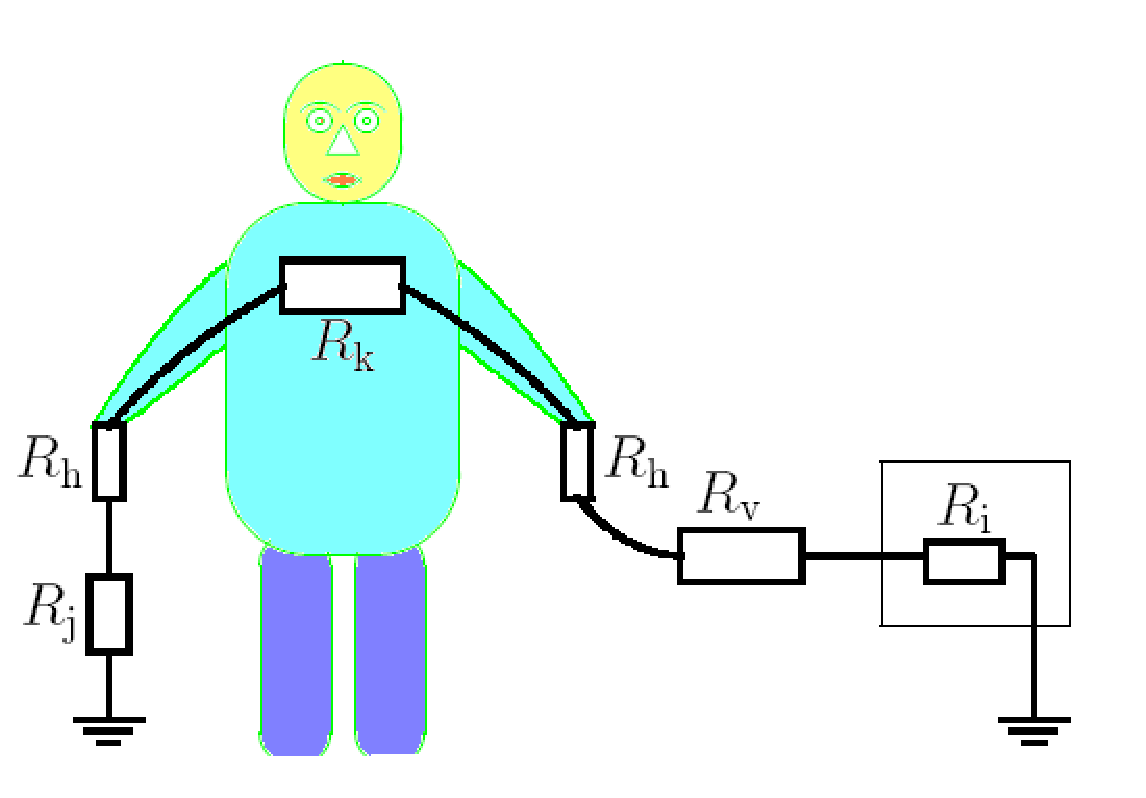
\includegraphics[width=10cm,height=6.96cm,keepaspectratio]{Kroppen_resized}
    \caption{
    Menneskekroppen som del av en strømkrets, hvor $R_\text{j}$ er isolasjonsmotstanden mellom kroppen og jord, $R_\text{h}$ er overgangsmotstanden i huden, $R_\text{k}$ er kroppens indre motstand, $R_\text{i}$ er indre motstand i spenningskilden som driver strømmen i kretsen og $R_\text{v}$ er isolasjonsmotstanden mellom spenningskildens spenningsterminal og kroppen.
    }
    \label{fig:Kroppen}
\end{figure}

Current passage can damage the body, either by damaging body tissue when heated, or by the current interfering with the electrical signals in the nervous system. The heating is given by the current $I$ and the resistance $R$ in the tissue being heated. A sustained flow through the tissue over time will add an increasing amount of heat energy and risk of injury. Disruption of the electrical signals in the nervous system can, among other things \, lead to heart fibrillation and paralysis. In particular, alternating current in the frequency range \num{15} to \SI{60}{\hertz} is dangerous for the nervous system. Our network supply of \SI{50}{\hertz} is therefore in the dangerous category. When the frequency of the alternating current increases, the influence on the nervous system will decrease, and for frequencies above \SI{10}{\kilo\hertz} the influence is almost gone. However, the heating effect is still present.

Current paths through the heart and lung region are particularly dangerous due to \ the vital organs that exist there. The kidneys are also particularly sensitive to current damage.

From the circuit in figure \ref{fig:Kroppen} we see that the current through the body is given by

\begin{equation}
    I = \frac{V}{R_\text{j} + 2R_\text{h} + R_\text{k} + R_\text{i} + R_\text{v}}.
    \label{eq:BodyVoltDiv}
\end{equation}

When referring to the voltage on a supply network, the effective value of the voltage, defined as

\begin{equation}
    V_\text{eff}
        = \sqrt{\langle V(t)^2 \rangle}
        = \sqrt{\frac{1}{T} \int_0^T V_0^2 \sin^2 \qty(\frac{2\pi t}{T}) \dd{t}}
        = \frac{V_0}{\sqrt{2}}.
    \label{eq:EffectiveV}
\end{equation}

This means that for a \num{230} volt system, the peak voltage (amplitude) is $V_0 = \sqrt{2} \times \SI{230}{\V} = \SI{325}{\V}$.

Safety precautions against electricity involve reducing the value of the current through the body to harmless values. This can be done for a given voltage $V$ by making sure that the sum of the resistances below the fractional line is sufficiently large:

\begin{itemize}
    \item [$R_\text{v}$] Ordinary electrical insulation of electrical equipment involves making $R_\text{v}$ sufficiently large.
    
%    \item[$R_\text{i}$] I laboppgaven i kapittel \ref{ch.coulomb} bruker du en \SI{12000}{\V} høyspenningskanon. Den blir ufarliggjort ved å gjøre $R_\text{i}$ så stor at $V/R_\text{i} < \SI{0,5}{\milli\ampere}$. 
    
    \item [$R_\text{k}$] The internal resistance of the body $R_\text{k}$ is constant and of the order of \SI{500}{\ohm}. Note that the limit for mandatory isolation of AC voltage of \SI{25}{\V} effective voltage corresponds to \SI{50}{\milli\ampere} when we assume that the resistance in the circuit consists only of the body's internal resistance, ie \ worst case.
    \item [$R_\text{h}$] The transition resistance $R_\text{h}$ in the skin can vary from \SI{0}{\ohm} for moist skin to well above \SI{10000}{\ohm} for dry skin. $R_\text{h}$ also decreases with increasing voltage and it also varies with the frequency so that it is lowest in the frequency range around \SI{50}{\hertz}. This helps to make AC voltage more dangerous than DC voltage. Another factor that makes alternating voltage more dangerous than direct voltage is that the magnitude of the voltage referred to when alternating voltage is mentioned is the effective voltage. However, the peak voltage is $\sqrt{2} \times $ higher, as described in equation \eqref{eq:EffectiveV}.
    \item [$R_\text{j}$] If the body is not in contact with the ground, $R_\text{j}$ will be large. Why do the birds not die when they are on power lines (see figure \ref{fig:BirdA})? Answer this question by modifying Figure \ref{fig:Kroppen}. Now look at figure \ref{fig:BirdB}, and then answer the question asked there.
    %Fugler som setter seg på høyspenningslinjer tar ikke skade p.g.a.\ at $R_{\rm j}$ er stor. Hvis handa di er i kontakt med en vannkran eller jordet ledning er $R_{\rm j} \approx 0 \; \Omega$.
\end{itemize}

\begin{figure}[!ht]
    \begin{minipage}[b]{0.49\linewidth}
        \centering
        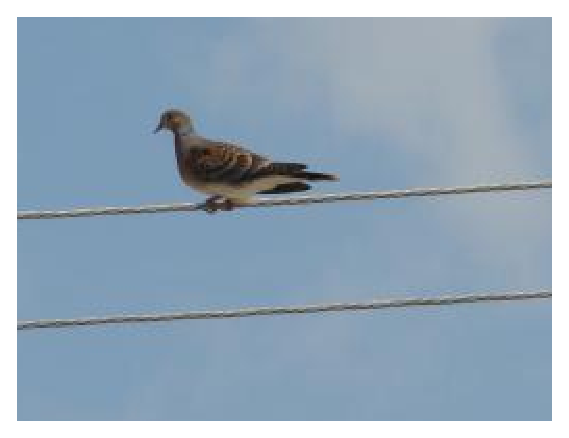
\includegraphics[scale=0.82]{fig/BirdL.eps}
        \caption{%
            En fugl som sitter på en kraftlinje.
        }
        \label{fig:BirdA}
    \end{minipage}
    \hspace{0.1cm}
    \begin{minipage}[b]{0.49\linewidth}
        \centering
        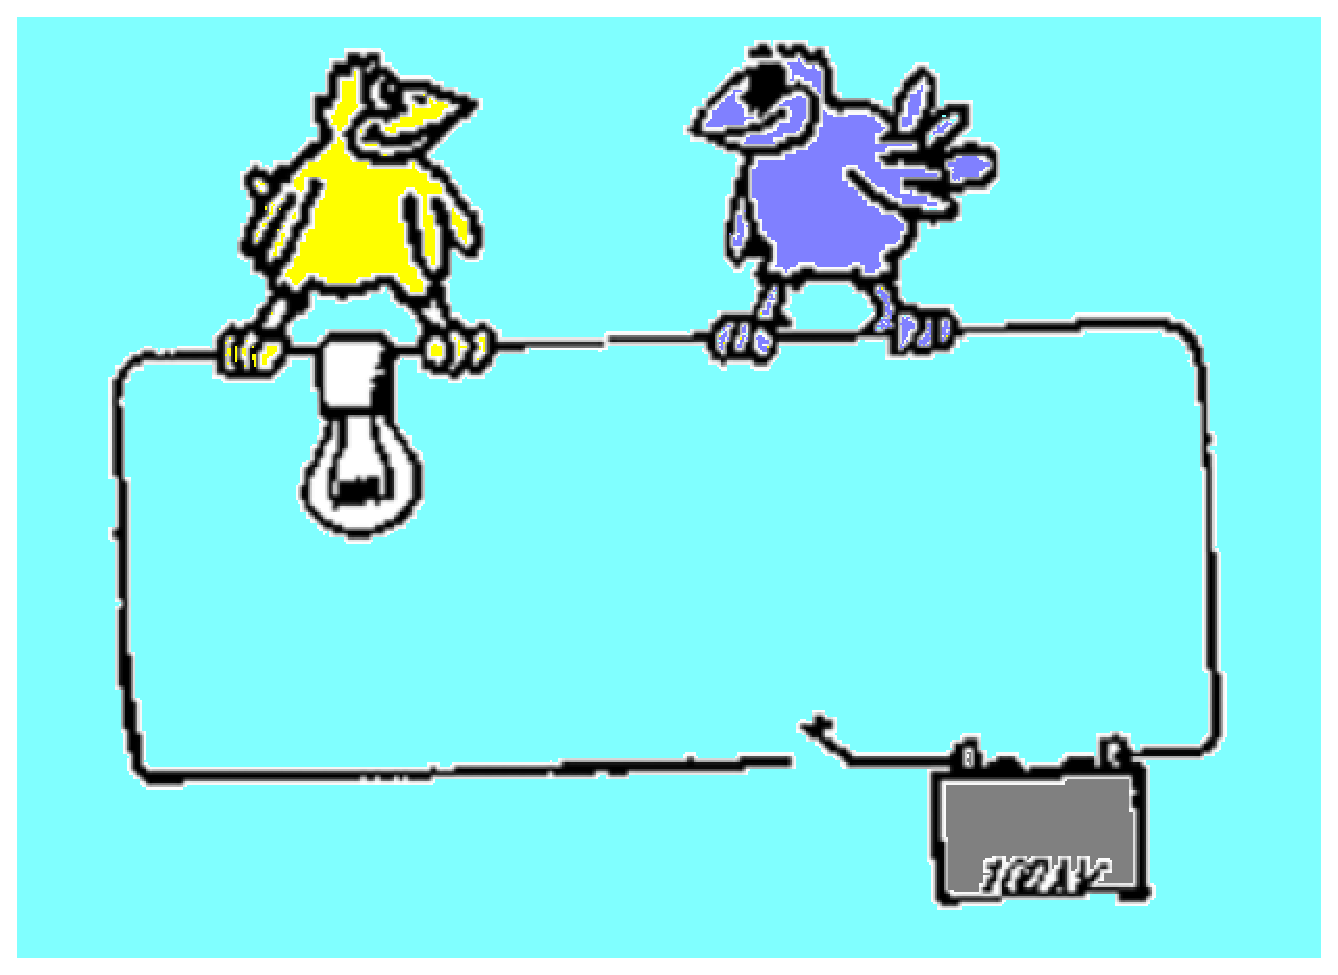
\includegraphics[scale=0.35]{fig/BirdC.eps}
        \caption{%
            Hva skjer når den slås på?
        }
        \label{fig:BirdB}
    \end{minipage}
\end{figure}

In addition to the above, it is important to be aware that high-frequency electromagnetic radiation in the \si{\mega\hertz} - \si{\giga\hertz} range (microwaves - radar) can be dangerous for the body in that the electric alternating field leads to heating of the body tissue, the same effect which provides heating in a microwave. Such high-frequency heating is extra dangerous because it often takes place without normal pain functions taking effect. Persons should be shielded if the power per unit area against the body is $> \SI{0,01}{\watt/\cm\squared}$.

\begin{table}[!ht]
    \begin{center}
    \caption{Limits of exposure\textsuperscript{a} to static magnetic fields}
    \label{tab:exposurlimits}
        \begin{tabular}{ l  c  c }
        \hline
        \noalign{\bigskip}
        \qquad\qquad Exposure characteristics &  & Magnetic flux density  \\
        \noalign{\medskip}
        \hline
        \noalign{\medskip}
        Occupational\textsuperscript{b} &  &  \\ 
        \noalign{\smallskip}
            \quad Exposure of head and trunk&   &  \SI{2}{\tesla} \\ 
            \quad Exposure of limbs\textsuperscript{c} & &  \SI{8}{\tesla}\\
        \noalign{\medskip}
        General public\textsuperscript{d} &  &  \\ 
        \quad Exposure of any part of the body& & \SI{400}{\milli\tesla}\\
        \noalign{\medskip}
        \hline
        \noalign{\medskip}
        \end{tabular}
    \end{center}
    \vspace*{-0.7cm}
\end{table}
%
\begin{figure}[!ht]
    \centering
    \begin{minipage}[t]{0.7\textwidth}
    \footnotesize{
        \textsuperscript{a} ICNIRP recommends that these limits should be viewed operationally as spatial peak exposure limits.\\
        \textsuperscript{b} For specific work applications, exposure up to \SI{8}{\tesla} can be justified, if the environment is controlled and appropriate work practices are implemented to control movement-induced effects.\\
        \textsuperscript{c} Not enough information is available on which to base exposure limits beyond \SI{8}{\tesla}.\\
        \textsuperscript{d} Because of potential indirect adverse effects, ICNIRP recognizes that practical policies need to be implemented to prevent inadvertent harmful exposure of persons with implanted electronic medical devices and implants containing ferromagnetic material, and dangers from flying objects, which can lead to much lower restriction levels such as \SI[output-decimal-marker = {.}]{0.5}{\milli\tesla}.
    }
    \end{minipage}
\end{figure}


%%%%%%%%%%%%%%%%%%%%%%%%%%%%%%%%
\section{Effect of static magnetic field}
%%%%%%%%%%%%%%%%%%%%%%%%%%%%%%%%
The International Commission on Non-Ionizing Radiation Protection (ICNIRP) provides in its guidelines recommended limit values   for exposure to electromagnetic fields (see Table \ref{tab:exposurlimits}). In Norway, the Radiation Protection Regulations stipulate that ICNIRP's guidelines must be followed, and that all exposure must be kept as low as practicable. For static magnetic fields, the recommended limit is \SI{2}{\tesla} for workers and \SI{400}{\milli\tesla} for the general population. Persons with pacemakers, ferromagnetic implants or implanted electronic components should not be exposed to magnetic fields above \SI{0,5}{\milli\tesla}. \footnote{\url{http://www.icnirp.de/documents/emfgdl.pdf} [\textit{Health Physics} \textbf{96} (2009) 504--519.]} In the experiment using the Helmholtz coils the magnetic flux density $B$ in the immediate vicinity of the coils has a value slightly exceeding \SI{0,5}{\milli\tesla} for $I = \SI{1}{\ampere}$ and $R = \SI{0,07}{\m}$, where $I$ is the current flowing in the coils and $R$ is the average radius of the coils . But the field decreases rapidly outside the coils; the magnitude of $B$ at a point perpendicular to the coil at a distance \SI{0,15}{\m} (or greater) from the center of the coil is less than \SI{50}{\micro\tesla}. If a current of \SI{0,5}{\ampere} is used, the field everywhere will be lower than the recommended limit for people with implants. A student with an implant that is sensitive to magnetic fields should inform the person in charge, who will ensure that this student has a partner who does not have an implant and that the partner makes the measurements.


%%%%%%%%%%%%%%%%%%%%%%%%%%%%%%%%
\section{Common sense in handling electrical equipment}
%%%%%%%%%%%%%%%%%%%%%%%%%%%%%%%%

In addition to the usual risks associated with electricity, some laboratories have high voltage equipment \footnote{For our purposes, it will be sufficient to consider any voltage higher than \SI{50}{\V} as high voltage.} Which poses an even greater potential hazard. Students should be extra careful with such equipment, and should learn how to disconnect the power source in an emergency. Here are some rules that must be followed when working with and near electricity.

\begin{enumerate}
    \item Do not work with electricity if your hands, feet, or other parts of your body are wet, or if you are standing on a wet floor.
    \item Inspect electrical equipment (with power off and unplugged) for broken wires and damaged connections. If such a thing is detected, do not use the equipment. Then report it to the person in charge so that the equipment can be repaired.
    \item Never attempt to repair electrical equipment yourself --- this must be done by qualified personnel.
    \item If you are subjected to even a mild shock from any equipment, it will be repaired immediately.
    \item Do not use or store extremely flammable liquids near electrical equipment. Some substances, such as ether, can be ignited by sparks from electrical equipment.
    \item Always use earthed sockets in earthed wall sockets. Never attempt to insert a grounded electrical outlet into an unearthed wall outlet.
    \item Extension cords should not be used instead of permanent wiring; they should only be used temporarily and they should not be pulled under doors, across hallways, through windows or holes in walls, around pipes or near sinks.
    \item Do not overload circuits by using branch outlets on a standard outlet.
    \item Do not remove or change safety measures on high voltage equipment. Remember they are there to protect you.
    \item Make sure that the power is switched off during connection or when making changes to the circuit.
    \item Make sure that all equipment is set with the correct settings according to the measurement to be performed before the circuit is made live.
    \item Make sure that the components used are of a rating that can withstand the applied current and voltage.
    \item Replace broken fuses with new ones of the correct type and with the correct specifications.
    \item {\itsf Hvis du tror noen har vært utsatt for et kraftig elektrisk sjokk\/}:
    \begin{itemize}
        \item do not remove the injured person from the electrical source until the power has been switched off.
        \item if you do not turn off the power, use an insulator such as a dry rope, cloth or broom handle to pull the person away from the power.
        \item check if there is contact.
        \item check if there is breathing.
        \item secure free airways.
        \item when injured do not breathe or in cardiac arrest, call 113 AMK control panel.
        \item provide cardiopulmonary resuscitation (CPR) 30 compressions and 2 breaths. Continue until healthcare professionals arrive.
        \item breathes the injured person himself, puts the person in a stable side position.
        \item look for burns and cool burns with water and treat them as third-degree burns.
        \item All injured persons must be supervised after first aid has been given. Do not leave unconscious persons. Conscious people should be talked to. Personal injuries must be treated further by medical personnel.
        \item persons sent to the Emergency Room by taxi / private car must be followed all the way in and out. Bring any HSE data sheets!
        \item all accidents / approaches to accidents are to be regarded as deviations in relation to normal operation, and must be reported on the deviation form.
    \end{itemize}
\end{enumerate}

In the experiment with Coulomb's law, the high-voltage cannon used to charge the bullets \SI{25}{\kilo\V} when activated. However, the current is limited to \SI{75}{\micro\ampere}. Such currents usually have no physiological effect on the body, but still: \textit{Behandle kanonen som om den var livsfarlig}.

\end{document}


